
% Probably cut most of this as redundant with 3710

{ % all template changes are local to this group.
    \setbeamertemplate{navigation symbols}{}
    \begin{frame}[plain]
        \begin{tikzpicture}[remember picture,overlay]
            \node[at=(current page.center)] {
                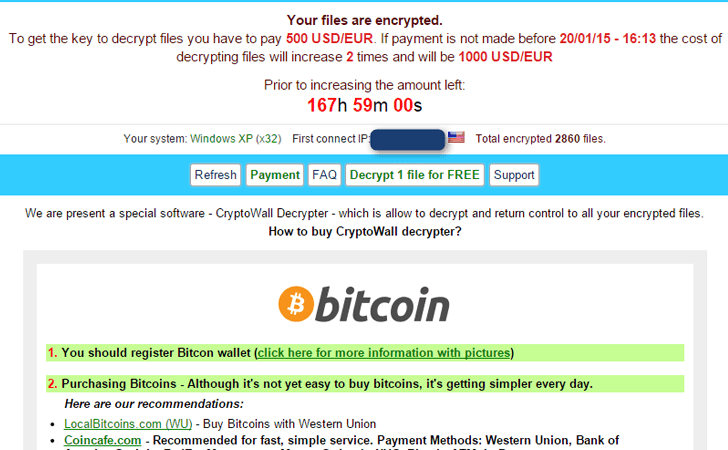
\includegraphics[width=\paperwidth]{../intro/cryptowall_ransom}
            };
        \end{tikzpicture}
    \end{frame}
}



% FIXME: davidson: 
    % examples of OPM, UVa, Colonial Pipeline hacks

% FIXME: https://arstechnica.com/security/2025/01/dozens-of-backdoored-chrome-extensions-discovered-on-2-6-million-devices/ 

\section{Malware and malware types}

\begin{frame}{malware}
    \begin{itemize}
    \item ``evil software''
    \item<2-> display a funny message
    \item<2-> send passwords/credit card numbers to criminals
    \item<2-> take pictures to send to criminals
    \item<2-> delete data
    \item<2-> hold data hostage
    \item<2-> insert/replace ads in webpages
    \item<2-> \ldots
    \end{itemize}
\end{frame}


\begin{frame}{viruses}
    \begin{itemize}
    \item malware that \myemph{inserts itself into another program}
    \item ``infects'' other programs when run
    \begin{itemize}
    \item usually modifies executables directly
    \end{itemize}
    \end{itemize}
\end{frame}

\begin{frame}{macro viruses}
    \begin{itemize}
    \item Word, Excel, other office software support \myemph{macros}
        \begin{itemize}
        \item scripts embedded in Word/Excel/etc. documents
        \end{itemize}
    \item viruses written in a \myemph{scripting language} 
        \begin{itemize}
        \item Visual Basic for Applications
        \end{itemize}
    \item spread to office documents, not executables
        \begin{itemize}
        \item easily spread in corporate environments
        \end{itemize}
    \item vendor reaction: macros disabled by default now
    \end{itemize}
\end{frame}

{ % all template changes are local to this group.
    \setbeamertemplate{navigation symbols}{}
    \begin{frame}[plain]
        \begin{tikzpicture}[remember picture,overlay]
            \node[at=(current page.center)] {
                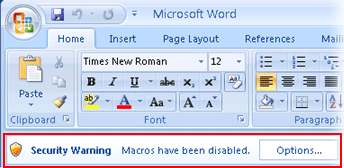
\includegraphics[width=\paperwidth]{../intro/msword-macro-warning}
            };
        \end{tikzpicture}
    \end{frame}
}

\begin{frame}{worms}
    \begin{itemize}
    \item \myemph{independent program}
    \item usually ``blends in'' with system programs
    \item copies itself to other machines or USB keys, etc.
    \item sometimes configures systems to run it automatically
    \end{itemize}
\end{frame}

\begin{frame}{trojan (horse)s}
    \begin{itemize}
    \item \myemph{useful-looking} program that is malware:
        \begin{itemize}
        \item `cracked' version of commerical software
        \item fake anti-virus software
        \item or looks like useful PDF doc
        \item \ldots
        \end{itemize}
    \item maybe is (or not), but also does something evil
    \item common form for targeted attacks
    \end{itemize}
\end{frame}

{ % all template changes are local to this group.
    \setbeamertemplate{navigation symbols}{}
    \begin{frame}[plain]
        \begin{tikzpicture}[remember picture,overlay]
            \node[at=(current page.center)] {
                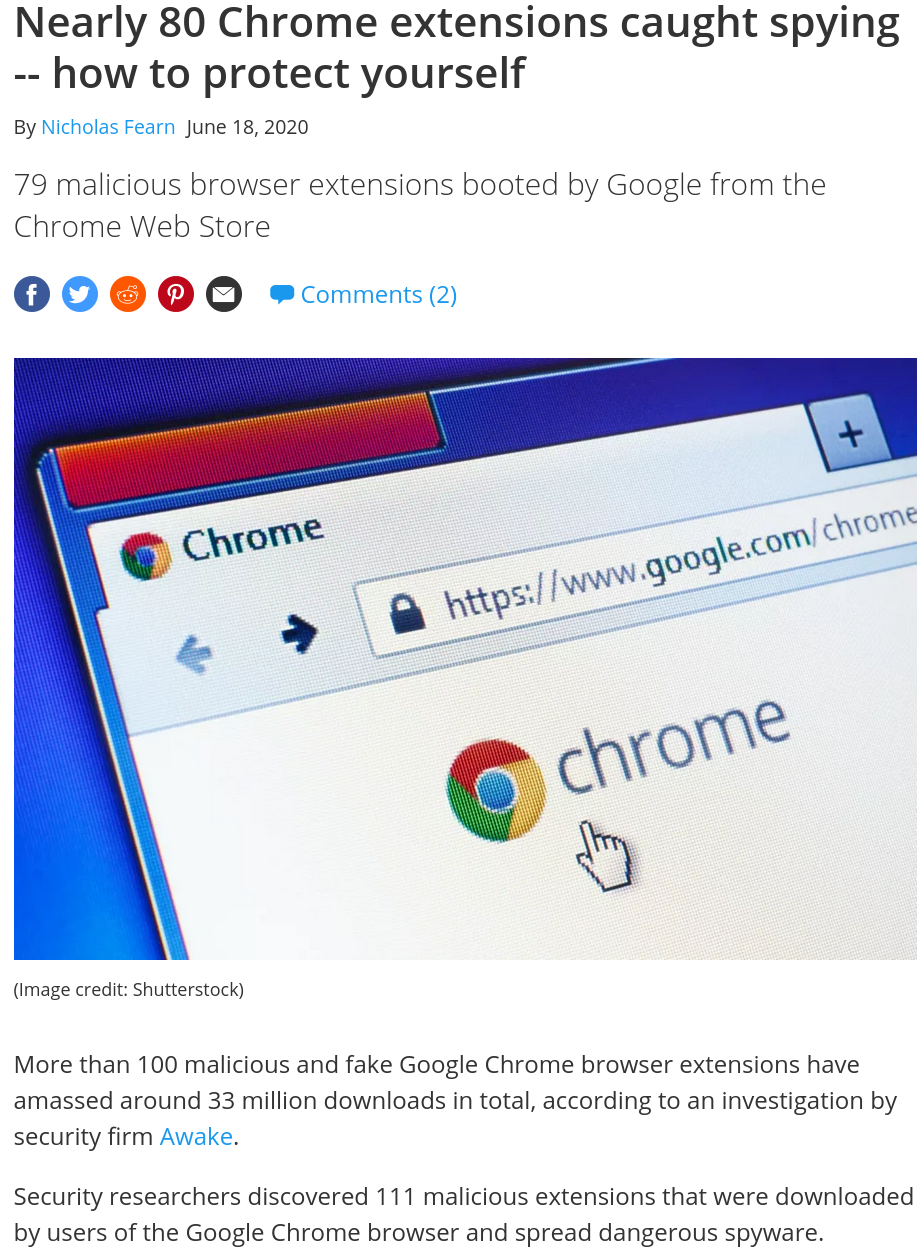
\includegraphics[height=\paperheight]{../intro/chrome-ext-article}
            };
        \end{tikzpicture}
    \end{frame}
}



\subsection{PUP}
\begin{frame}{potentially unwanted programs (PUP)}
    \begin{itemize}
    \item most commonly: programs bundled with other programs
    \item sometimes disclosed but in (deceptive?) fine print
    \item sometimes considered malware, sometimes not
    \end{itemize}
\end{frame}

\begin{frame}{bad behavior by `normal' programs}
    \begin{itemize}
    \item some mostly-legitimate programs also do malware-like things
    \vspace{.5cm}
    \item location info collected by cell phone apps?
    \item advertisments injected by useful browser extensions?
    \end{itemize}
\end{frame}


{ % all template changes are local to this group.
    \setbeamertemplate{navigation symbols}{}
    \begin{frame}[plain]
        \begin{tikzpicture}[remember picture,overlay]
            \node[at=(current page.center)] {
                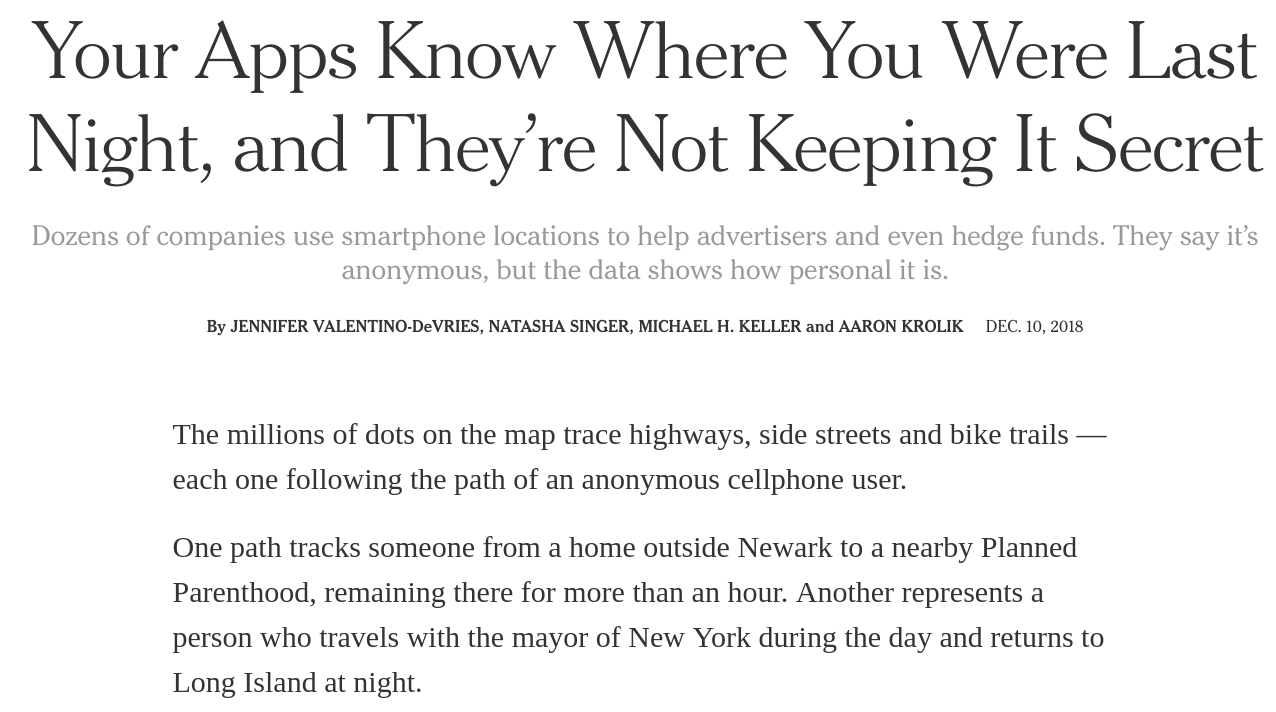
\includegraphics[width=\paperwidth]{../intro/app-location-data-art}
            };
        \end{tikzpicture}
    \end{frame}
}


\subsection{Web malware locations}
\usetikzlibrary{calc}
\begin{frame}

\includegraphics[width=\textwidth]{../intro/kotzias-on-device-title}
\end{frame}

\begin{frame}
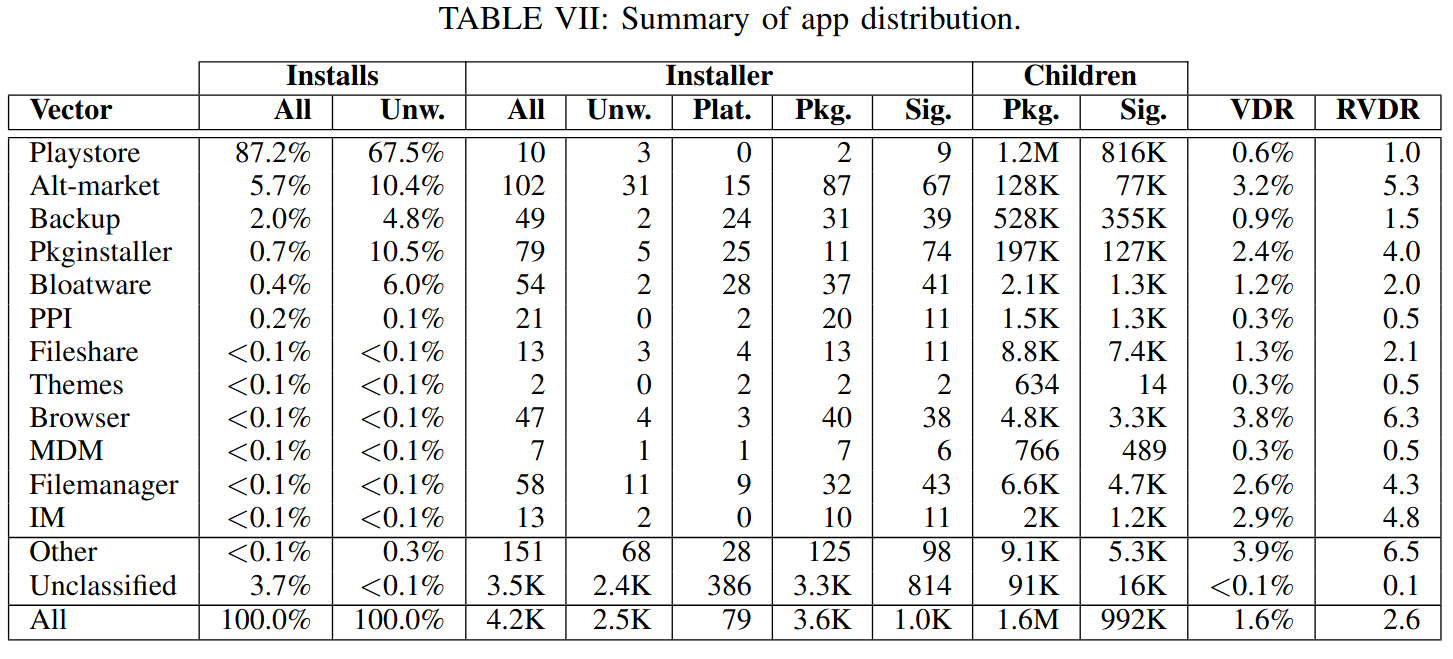
\includegraphics[width=\textwidth]{../intro/kotzias-install-src-tbl}
\imagecredit{VDR=portion detected as unwanted; PPI=pay-per-install; MDM=mobile device management}
\end{frame}



\subsection{exercise/discussion}
\begin{frame}{what is malware\ldots}
\begin{itemize}
\item opinion question: \\
if you're making anti-malware software, what should it do for\ldots?
    \begin{itemize}
    \item (1) pre-installed browser extension that displays coupon codes \\
          but sends domain name of all websites to third-party to do so
          \vspace{.25cm}
    \item (2) remote administration software that shows a subtle icon \\
          in the corner of the screen when used to monitor the machine
    \end{itemize}
\vspace{.5cm}
\item A. remove it, no prompting
\item B. prompt to remove it, default to yes
\item C. prompt to remove it, default to no
\item D. don't flag it
\item E. something else (discuss?)
\end{itemize}
\end{frame}


\subsection{stalkerware, dual-use software}

{
    \begin{frame}[plain]
        \begin{tikzpicture}[remember picture,overlay]
            \node[at=(current page.north),anchor=north] (head){
                
\includegraphics[width=0.9\paperwidth]{../intro/ipv-spyware-paper-head}
            };
            \node[at={([yshift=5mm]current page.south)},anchor=south] {
                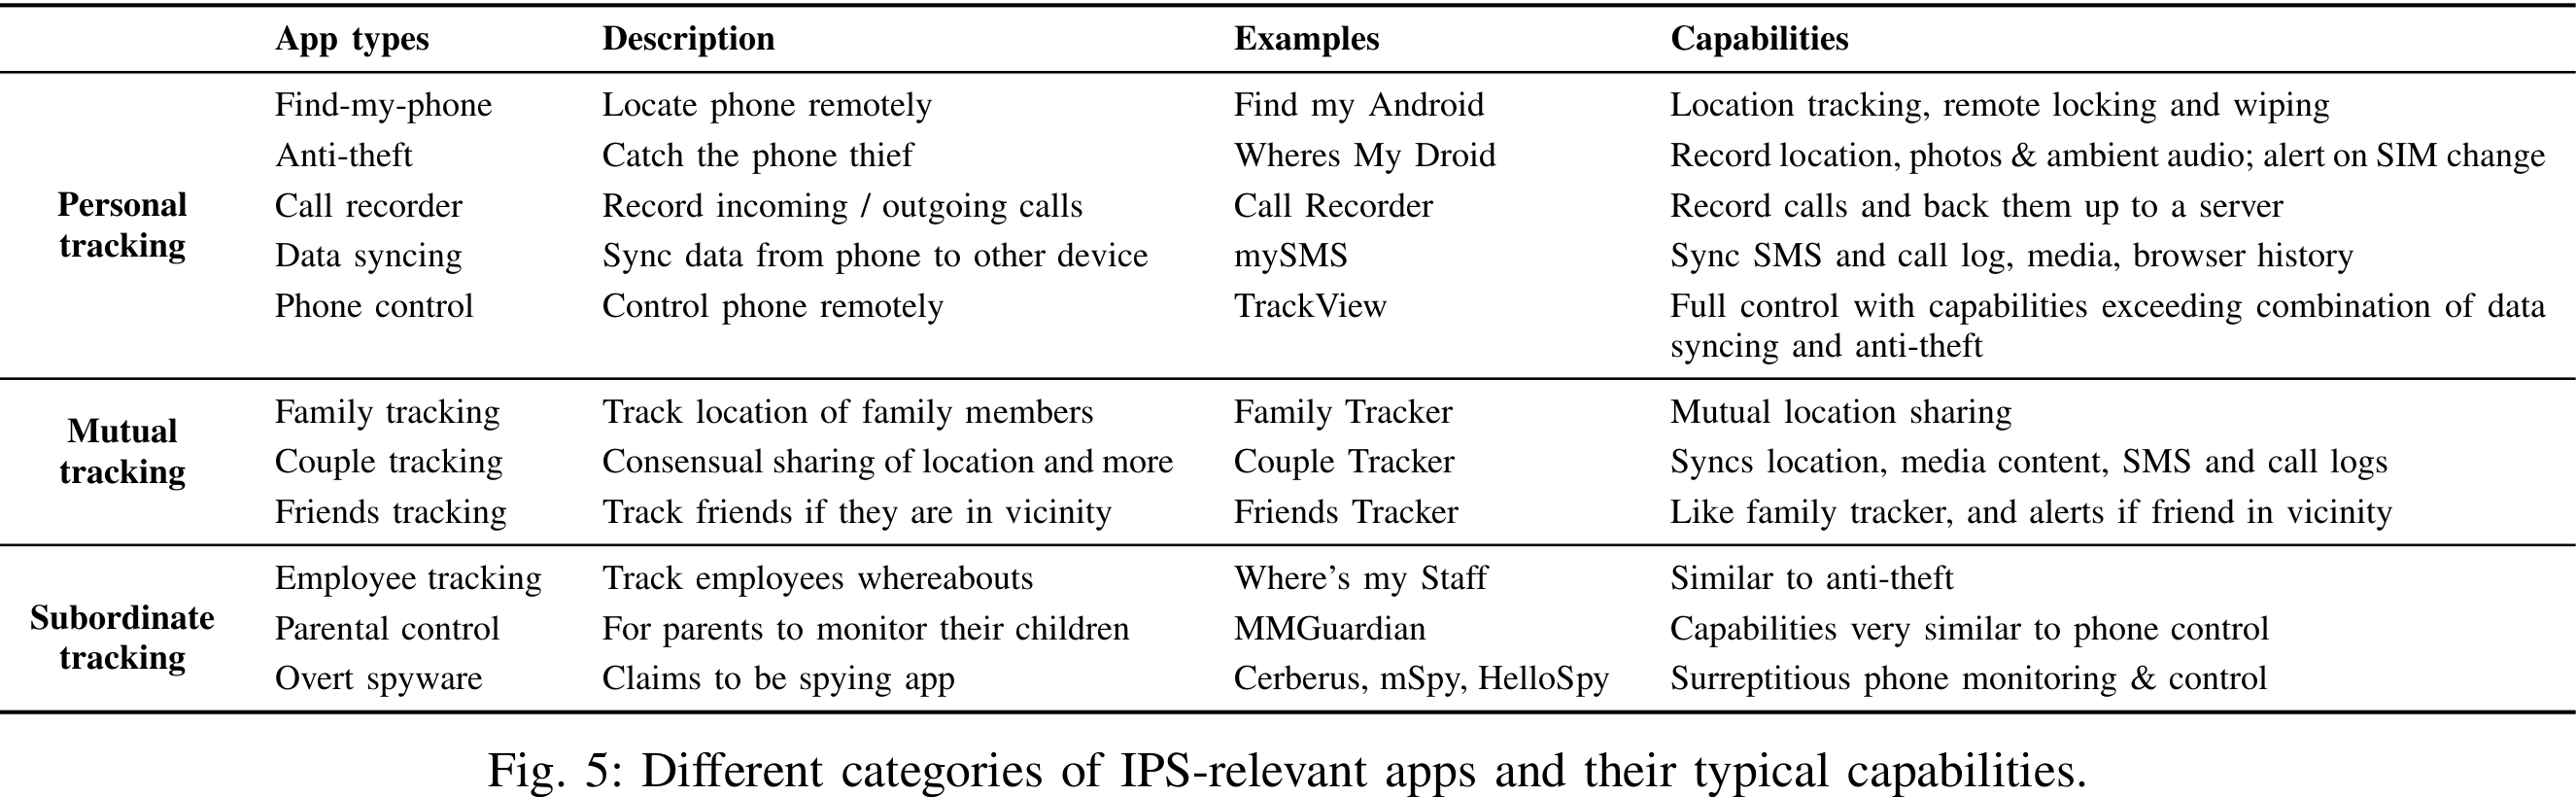
\includegraphics[width=0.98\paperwidth]{../intro/ipv-spyware-types}
            };
        \end{tikzpicture}
    \end{frame}
}

\begin{frame}{dual-use, context-sensitivity}
    \begin{itemize}
    \item this class: mostly talking about clearly anti-user software
        \begin{itemize}
        \item \ldots and how it tries to be covert
        \end{itemize}
    \vspace{.5cm}
    \item but there are also problems of \textit{dual-use} software
        \begin{itemize}
        \item phone tracking anti-theft software
        \item computer remote administration software
        \end{itemize}
    \item (also problems of intentionally `evil' software masquarding as legit)
        \begin{itemize}
        \item (e.g. marketted on ``how to spy on your \rule{1cm}{.5pt}'' blog)
        \item (e.g. unnecessairily well hidden when installed)
        \end{itemize}
    \item ideally, prevent ``bad'' use somehow
        \begin{itemize}
        \item phone OS should prevent \textit{covert} tracking?
        \item antimalware software should notice such software?
        \item \ldots
        \end{itemize}
    \end{itemize}
\end{frame}


\section{follow the money}
\begin{frame}<1>[label=followTheMoney]{making money from malware}
    \begin{itemize}
    \item often malware authors trying to make money
    \vspace{.5cm}
    \item \myemph<2>{adware --- from ad revenue}
    \item \myemph<3>{ransomware --- ransom user's files/usability of system}
    \item \myemph<5>{resell personal info}
    \item \myemph<4>{resell computation/network time}
        \begin{itemize}
        \item advertising fraud
        \item distributed denial of service
        \item cryptocurrency minining
        \end{itemize}
    \end{itemize}
\end{frame}


\subsection{Malware Types?}
\usetikzlibrary{calc}

\begin{frame}{aside on malware statistics}
    \begin{itemize}
    \item most malware statistics come from antivirus companies
    \item probably a biased data source
    \end{itemize}
\end{frame}

{
    \setbeamertemplate{navigation symbols}{}
    \begin{frame}[plain]
        \begin{tikzpicture}[remember picture,overlay]
            \node[at=(current page.center)] {
                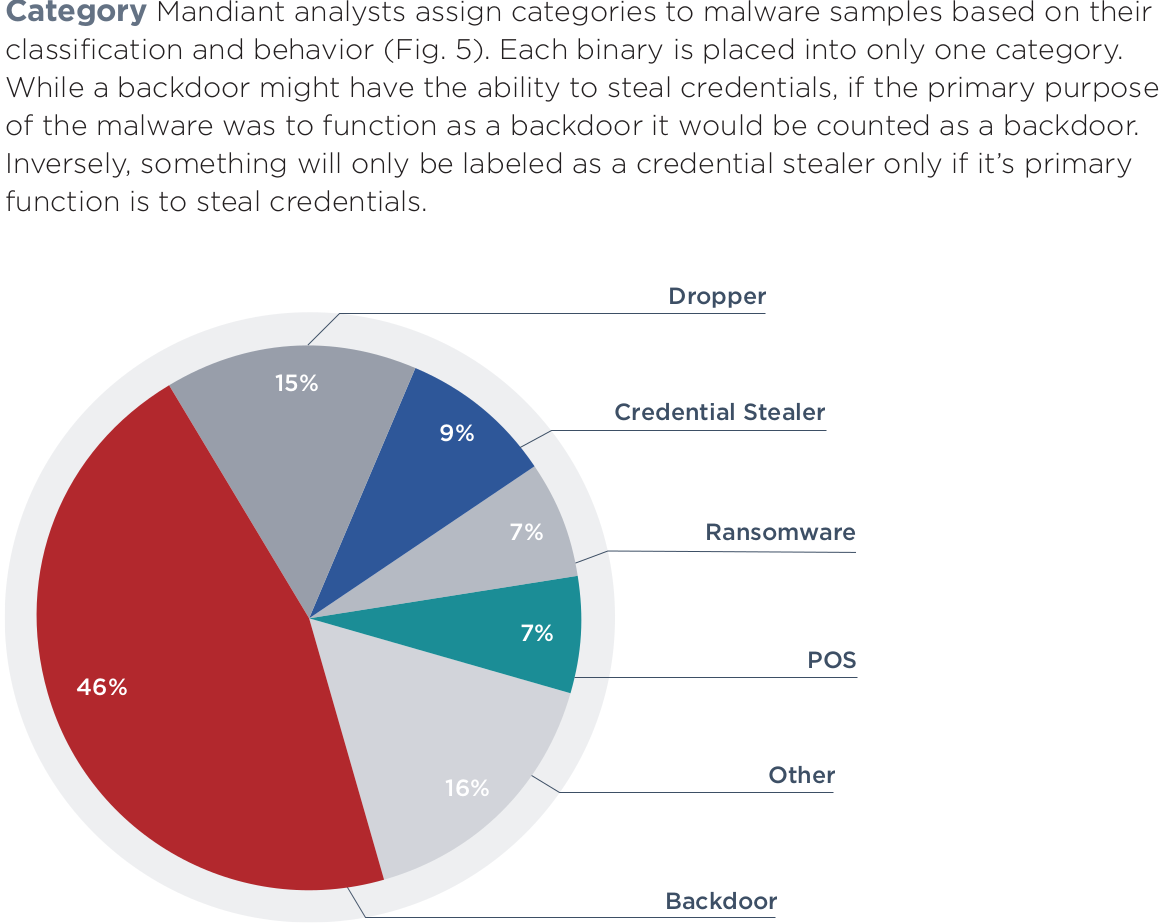
\includegraphics[height=0.95\textheight]{../intro/fireeye-malware-types-cut}
            };
        \end{tikzpicture}
        \imagecredit{Source: FireEye M-Trends Report 2020}
    \end{frame}
}



\subsection{Pay-Per-Install}
{
    \setbeamertemplate{navigation symbols}{}
    \begin{frame}[plain]
        \begin{tikzpicture}[remember picture,overlay]
            \node[at=(current page.center)] {
                
\includegraphics[width=\textwidth]{../intro/ppi-title}
            };
        \end{tikzpicture}
    \end{frame}
}

{
    \setbeamertemplate{navigation symbols}{}
    \begin{frame}[plain]
        \begin{tikzpicture}[remember picture,overlay]
            \node[at=(current page.center)] {
                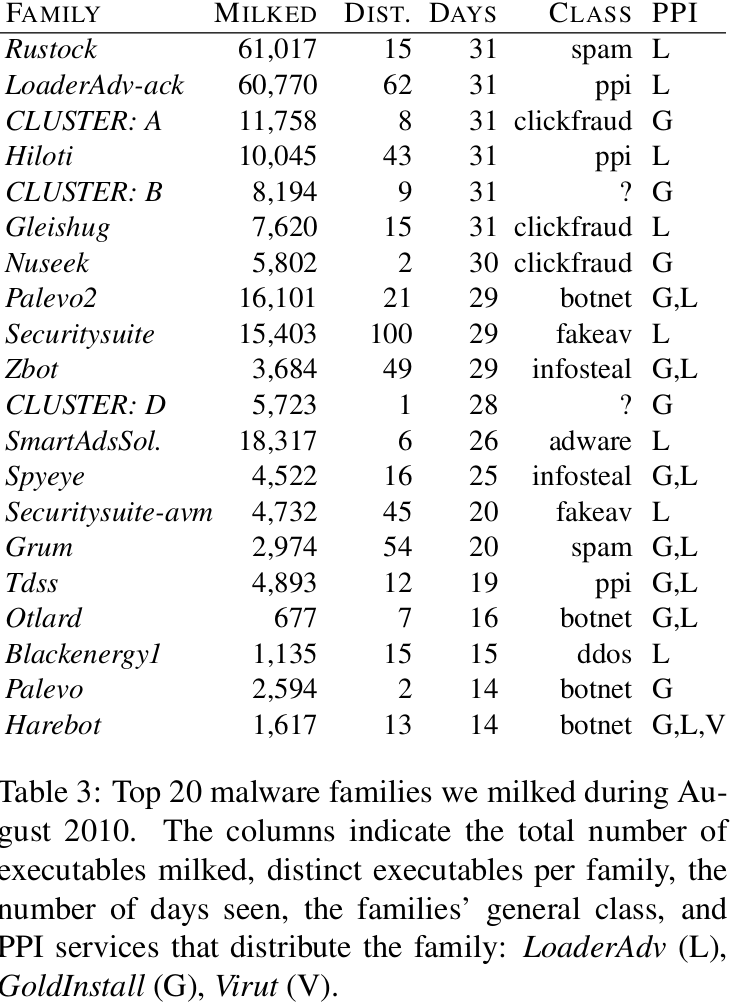
\includegraphics[height=\textheight]{../intro/ppi-top-20b}
            };
        \end{tikzpicture}
    \end{frame}
}



\subsection{Adware}
\againframe<2>{followTheMoney}
\usetikzlibrary{calc}
\begin{frame}{ad injection (1)}
    \begin{itemize}
        \item internet advertising is big business
        \item \ldots{} but you need to pay websites to add ads?
        \item how about \myemph{modifying browser} to add/change ads
        \vspace{.5cm}
        \item mostly \myemph{bundled} with legitimate software
    \end{itemize}
\end{frame}


{ % all template changes are local to this group.
    \setbeamertemplate{navigation symbols}{}
    \begin{frame}[plain]
        \begin{tikzpicture}[remember picture,overlay]
            \node[at=(current page.center)] {
                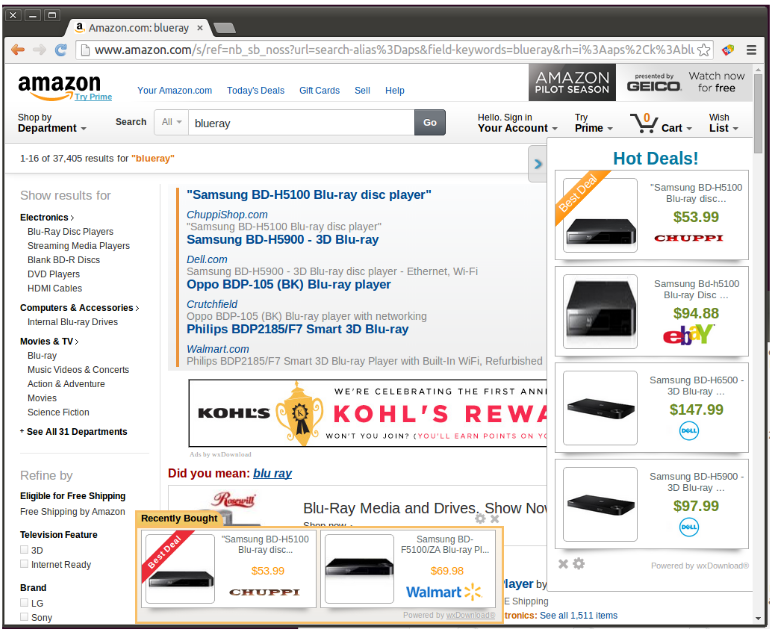
\includegraphics[height=0.96\paperheight]{../intro/ad-inject-amazon}
            };
        \end{tikzpicture}
    \imagecredit{From Thomas et al, ``Ad Injection at Scale: Assessing Deceptive Advertisement Modifications''}
    \end{frame}
}

\begin{frame}{ad injection (2)}
    \begin{itemize}
        \item 5\% of Google-accessing clients (2014)
        \item >90\% using code from VC-backed firm SuperFish:
        \vspace{.5cm}
            \item \$19.3 M in investment (CrunchBase)
            \item \$38M in revenue (Forbes, 2015)
            \item defunct after Lenovo root CA incident (2015)
            \item \ldots{} but founders reported started new, similar venture (JustVisual; according to TechCrunch)
    \end{itemize}
    \imagecredit{Adware prevalence: Thomas et al, ``Ad Injection at Scale: Assessing Deceptive Advertisement Modifications''}
\end{frame}



% FIXME: reselling info
\subsection{Reselling Info}
\begin{frame}[plain]
\begin{tikzpicture}[overlay,remember picture]
\node[anchor=north west,at={(current page.north west)}] (zdnet logo) {
    
\includegraphics[width=0.08\paperwidth]{../intro/ad-blocker-zdnet-logo2}
};
\node[anchor=north east,at={(current page.north east)}] (title) {
    
\includegraphics[width=0.9\paperwidth]{../intro/ad-blocker-user-data-title}
};
\node[anchor=north,at={(title.south)}] (author) {
    
\includegraphics[width=0.9\paperwidth]{../intro/ad-blocker-author}
};
\node[anchor=north,at={([yshift=-2cm]author.south)}] {
    
\includegraphics[width=0.9\paperwidth]{../intro/ad-blocker-user-data-quote}
};
\end{tikzpicture}
\end{frame}


\subsection{Ransomware: cryptolockers}
\againframe<3>{followTheMoney}

\begin{frame}{cryptolockers}
    \begin{itemize}
        \item encrypt files, hold for ``ransom''
        \item decryption key stored only on attacker-controlled server
        \item possibly decrypt files if victim pays
        \vspace{.5cm}
        \item many millions in revenues 
        \begin{itemize}
            \item accurate numbers are hard to find
        \end{itemize}
    \end{itemize}
\end{frame}


{ % all template changes are local to this group.
    \setbeamertemplate{navigation symbols}{}
    \begin{frame}[plain]
        \begin{tikzpicture}[remember picture,overlay]
            \node[at=(current page.center)] {
                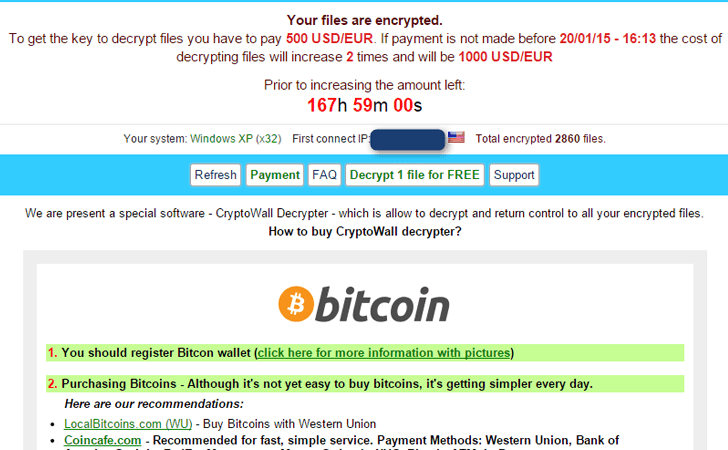
\includegraphics[width=\paperwidth]{../intro/cryptowall_ransom}
            };
        \end{tikzpicture}
    \end{frame}
}



\begin{frame}{other ransomware}
    \begin{itemize}
    \item we have your private data, pay us or it gets released
    \end{itemize}
\end{frame}


\subsection{targetting / other extortion}
\begin{frame}{more targetted stealing/extortion}
\end{frame}


{
    \setbeamertemplate{navigation symbols}{}
    \begin{frame}[plain]
        \begin{tikzpicture}[remember picture,overlay]
            \node[at=(current page.north),anchor=north] {
                
\includegraphics[width=0.8\paperwidth]{../intro/catch-ratter-title}
            };
            \node[at=(current page.south),anchor=south] {
                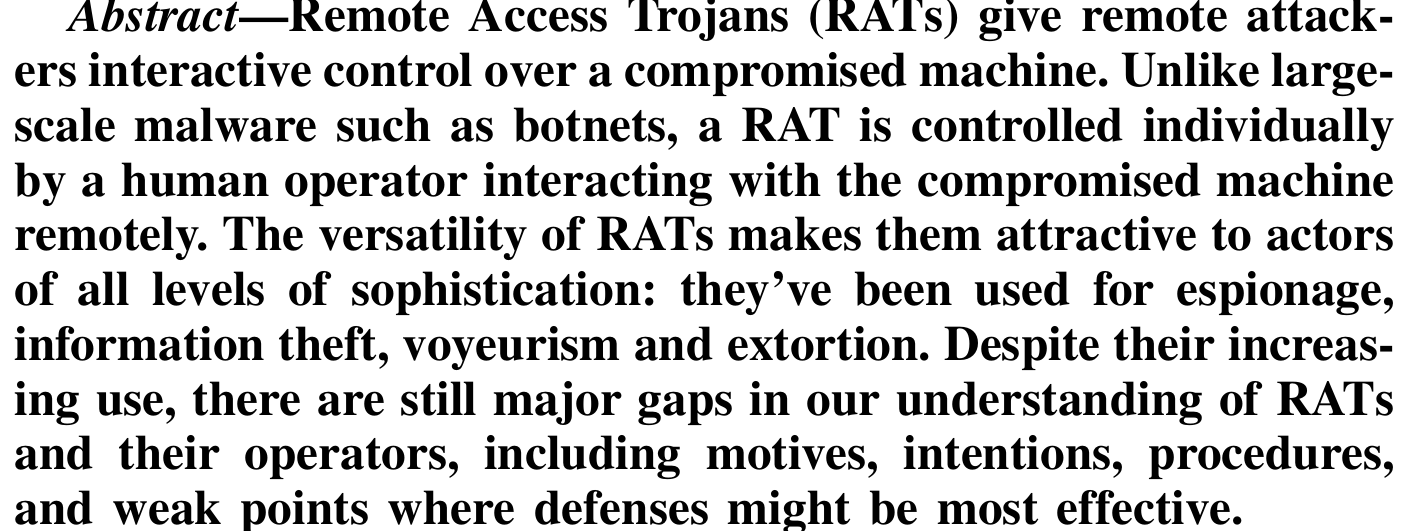
\includegraphics[height=0.5\paperheight]{../intro/catch-ratter-abs1}
            };
        \end{tikzpicture}
    \end{frame}
}

\begin{frame}{to catch ratter results}
    \begin{itemize}
    \item 2016/7 study
    \item 61\% attempt to access webcam; 26\% microphone
        \begin{itemize}
        \item (both not present in experimenter's `honeypot')
        \end{itemize}
    \item 31\% enable keylogger (passwords?)
    \item approx. 5\% harass legit user
    \item approx. 2\% try to phish legit user
    \end{itemize}
\end{frame}



\subsection{black markets, generally}
\begin{frame}[fragile,label=underground1]{the underground economy (1)}
\begin{tikzpicture}[overlay,remember picture]
\node[anchor=center,draw,very thick] (quote) at (current page.center) {
    
\includegraphics[width=0.9\textwidth]{../intro/bm-sell-cvv}
};
\node[font=\fontsize{11}{12}\selectfont,anchor=north,align=left] (quote explain) at (quote.south){
        advertisment for stolen credentials on an IRC (Internet Relay Chat) server \\
        via Team Cymru, ``The underground Economy: Priceless'' (2006, Usenix ;login: magazine)
    };
    \node[font=\fontsize{11}{12}\selectfont,anchor=north west,align=left] at (quote explain.south west) {
        (CVV = card verification value --- verification number on back of credit cards) \\
        (DL = driver's license?)
    };
\end{tikzpicture}
\end{frame}

\begin{frame}[fragile,label=underground2]{the underground economy (2)}
\begin{tikzpicture}[overlay,remember picture]
\node[anchor=center,draw,very thick] (quote) at (current page.center) {
    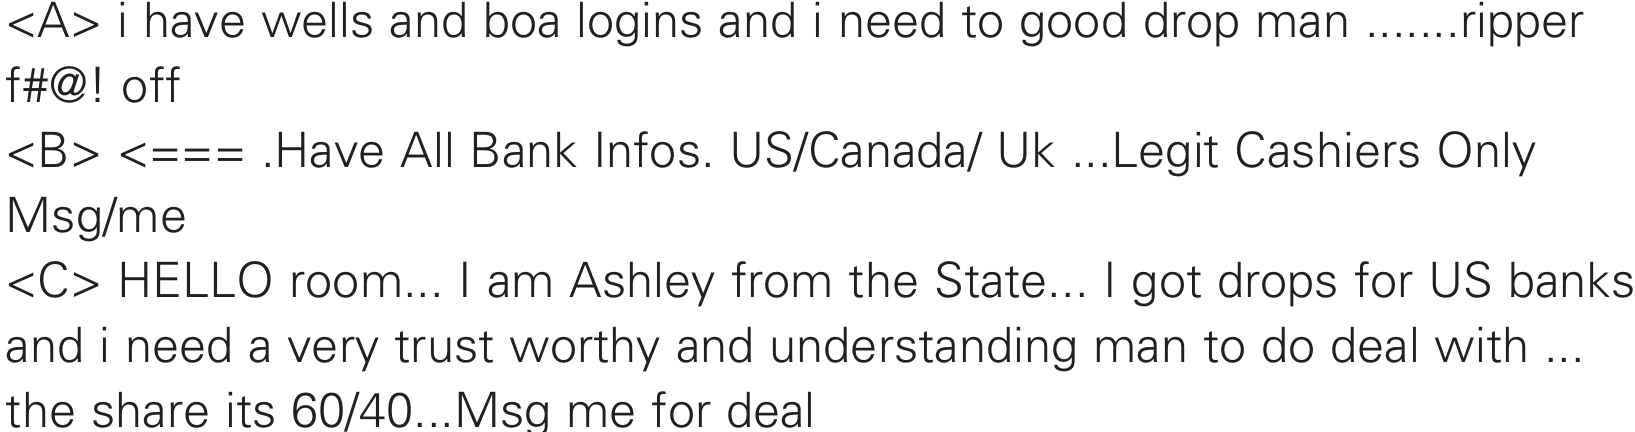
\includegraphics[width=0.9\textwidth]{../intro/underground-dropscashiers}
};
\node[font=\fontsize{11}{12}\selectfont,anchor=north,align=left] (quote explain) at (quote.south){
        advertisements for `drops' (bank accounts for money laundering) and \\
        for `cashiers' (criminals who will clean out accounts) \\
        via Team Cymru, ``The underground Economy: Priceless'' (2006, Usenix ;login: magazine)
    };
\end{tikzpicture}
\end{frame}

\begin{frame}[fragile,label=underground3]{the underground econmomy (3)}
\begin{tikzpicture}[overlay,remember picture]
\node[anchor=center,draw,very thick] (taxonomy) at (current page.center) {
    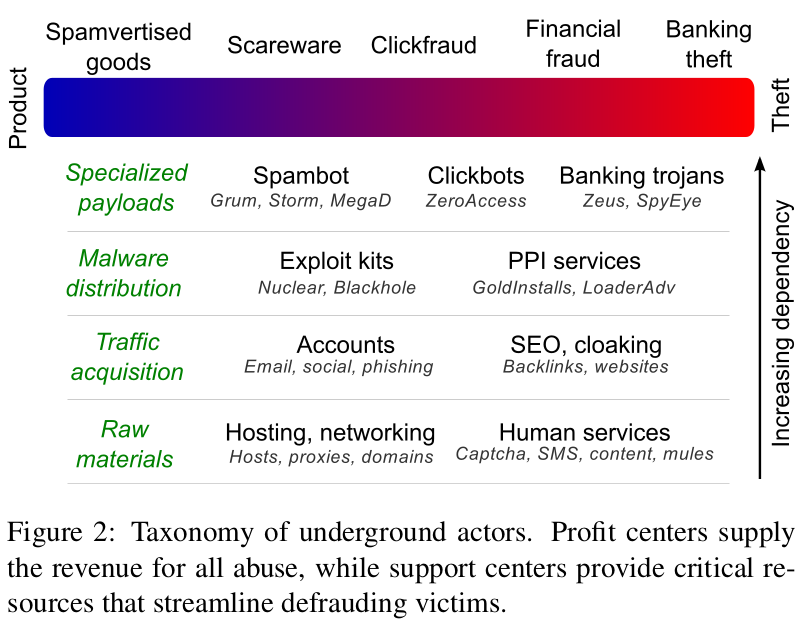
\includegraphics[width=0.9\textheight]{../intro/taxonomy-underground}
};
\node[font=\fontsize{11}{12}\selectfont,anchor=north,align=left] (explain) at (taxonomy.south){
    via Thomas et al, ``Framing Dependencies Introduced by Underground Commoditization'' (2015)
};
\end{tikzpicture}
\end{frame}


\subsection{espinoge}
\begin{frame}{targeted attacks / espionage}
    \begin{itemize}
    \item information gathering
        \begin{itemize}
        \item SolarWinds (network monitoring software) attack (``supply chain'')
        \item exploits via subject-specific links (``here's an interesting PDF'')
        \end{itemize}
    \item sabotage
        \begin{itemize}
        \item Stuxnet: Iranian enrichment controls
        \end{itemize}
    \end{itemize}
\end{frame}


\subsubsection{SolarWinds}
\begin{frame}{SolarWinds}
    \begin{itemize}
    \item supplier of network-monitoring software
    \item \ldots used by many big customers, including US Gov't
    \vspace{.5cm}
    \item attacked by third-party to spy (?) on customers
    \end{itemize}
\end{frame}


\subsubsection{Stuxnet}

\begin{frame}{Stuxnet}
    \begin{itemize}
        \item targeted Iranian nuclear enrichment facilities
        \item physically damaged centrifuges
        \item designed to spread via USB sticks
        \item publicly known 2010, deployed 2009
        \item US + Israel gov't developed
            \begin{itemize}
            \item according to press reports
            \end{itemize}
    \end{itemize}
\end{frame}




\subsection{Note on attacking monetization}

\begin{frame}{why talk about why/what?}
    \begin{itemize}
    \item doesn't change malware much
    \item (also, not a likely topic later in this course)
    \item \ldots but\ldots
    \vspace{.5cm}
    \item attacking monetization/other goals often effective\ldots
    \item may be more effective than our focus on exploits/code/etc.
    \end{itemize}
\end{frame}


\section{Software vulnerabilities, versus exploit}


\begin{frame}{vulnerabilities}
    \begin{itemize}
    \item for viruses, worms
    \item for trojans + PUP that do more than is supposed to do be allowed
        \begin{itemize}
        \item e.g. getting location information without ``permission''
        \end{itemize}
    \vspace{.5cm}
    \item software \myemph{vulnerability}
    \vspace{.5cm}
    \item unintended program behavior \\ that can be used by an adversary
    \end{itemize}
\end{frame}

\begin{frame}{vulnerability example}
    \begin{itemize}
    \item website able to install software without prompting
    \item \myemph{not intended} behavior of web browser
    \end{itemize}
\end{frame}


\begin{frame}{software vulnerability classes (1)}
    \begin{itemize}
    \item \myemph{memory safety} bugs
        \begin{itemize}
        \item problems with pointers
        \item big topic in this course
        \end{itemize}
    \item ``injection'' bugs --- \myemph{type confusion}
        \begin{itemize}
        \item commands/SQL within name, label, etc.
        \end{itemize}
    \item integer overflow/underflow
    \item \ldots
    \end{itemize}
\end{frame}

\begin{frame}{software vulnerability classes (2)}
    \begin{itemize}
    \item not checking inputs/permissions
        \begin{itemize}
        \item \url{http://webserver.com/../../../../file-I-shouldn't-get.txt}
        \end{itemize}
    \item almost any ``undefined behavior'' in C/C++
    \item synchronization bugs: time-to-check to time-of-use
    \item \ldots{} more?
    \end{itemize}
\end{frame}

\begin{frame}{vulnerability versus exploit}
    \begin{itemize}
    \item exploit --- something that uses a vulnerability to do something
    \item proof-of-concept --- something = demonstration the exploit is there
        \begin{itemize}
        \item example: open a calculator program
        \end{itemize}
    \end{itemize}
\end{frame}




\section{Malware spreading}

\begin{frame}{malware spreading with human help}
    \begin{itemize}
    \item installed by other malware
    \item installed manually after illegitimate access
    \item including in deceptively marketted software
    \end{itemize}
\end{frame}




\begin{frame}{malware spreading without human help}
    \begin{itemize}
        \item vulnerable network-accessible services
        \item shared files/folders  
            \begin{itemize}
            \item autorun on USB sticks
            \item macros in Word/Excel/etc. files
            \end{itemize}
        \item email attachments
        \item websites + browser vulnerabilities
            \begin{itemize}
            \item JavaScript interpreter bugs
            \item Adobe Flash Player bugs
            \end{itemize}
    \end{itemize}
\end{frame}




\section{Defenses}

\begin{frame}{malware defenses (1)}
    \begin{itemize}
        \item ``antivirus'' software:
        \vspace{.5cm}
        \item Windows Defender
        \item avast!
        \item Avira
        \item AVG
        \item McAfee
        \item \ldots
    \end{itemize}
\end{frame}

\begin{frame}{malware defenses (2)}
    \begin{itemize}
        \item app stores/etc. filtering (in theory)
            \begin{itemize}
            \item require developer registration
            \item program analysis?
            \item blacklisting after the fact?
            \end{itemize}
        \item ``sandboxing'' policies
            \begin{itemize}
            \item don't let, e.g., game access your taxes
            \item don't let weather app access your microphone
            \end{itemize}
    \end{itemize}
\end{frame}

\begin{frame}[plain]
    \begin{tikzpicture}[remember picture,overlay]
        \node[at=(current page.center)] {
            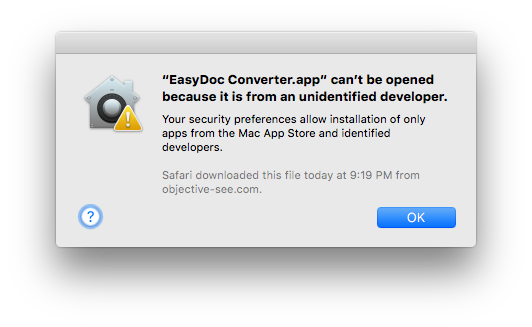
\includegraphics[width=\paperwidth]{../intro/app-denied-mac}
        };
    \end{tikzpicture}
\end{frame}

\begin{frame}[plain]
    \begin{tikzpicture}[remember picture,overlay]
        \node[at=(current page.center)] {
            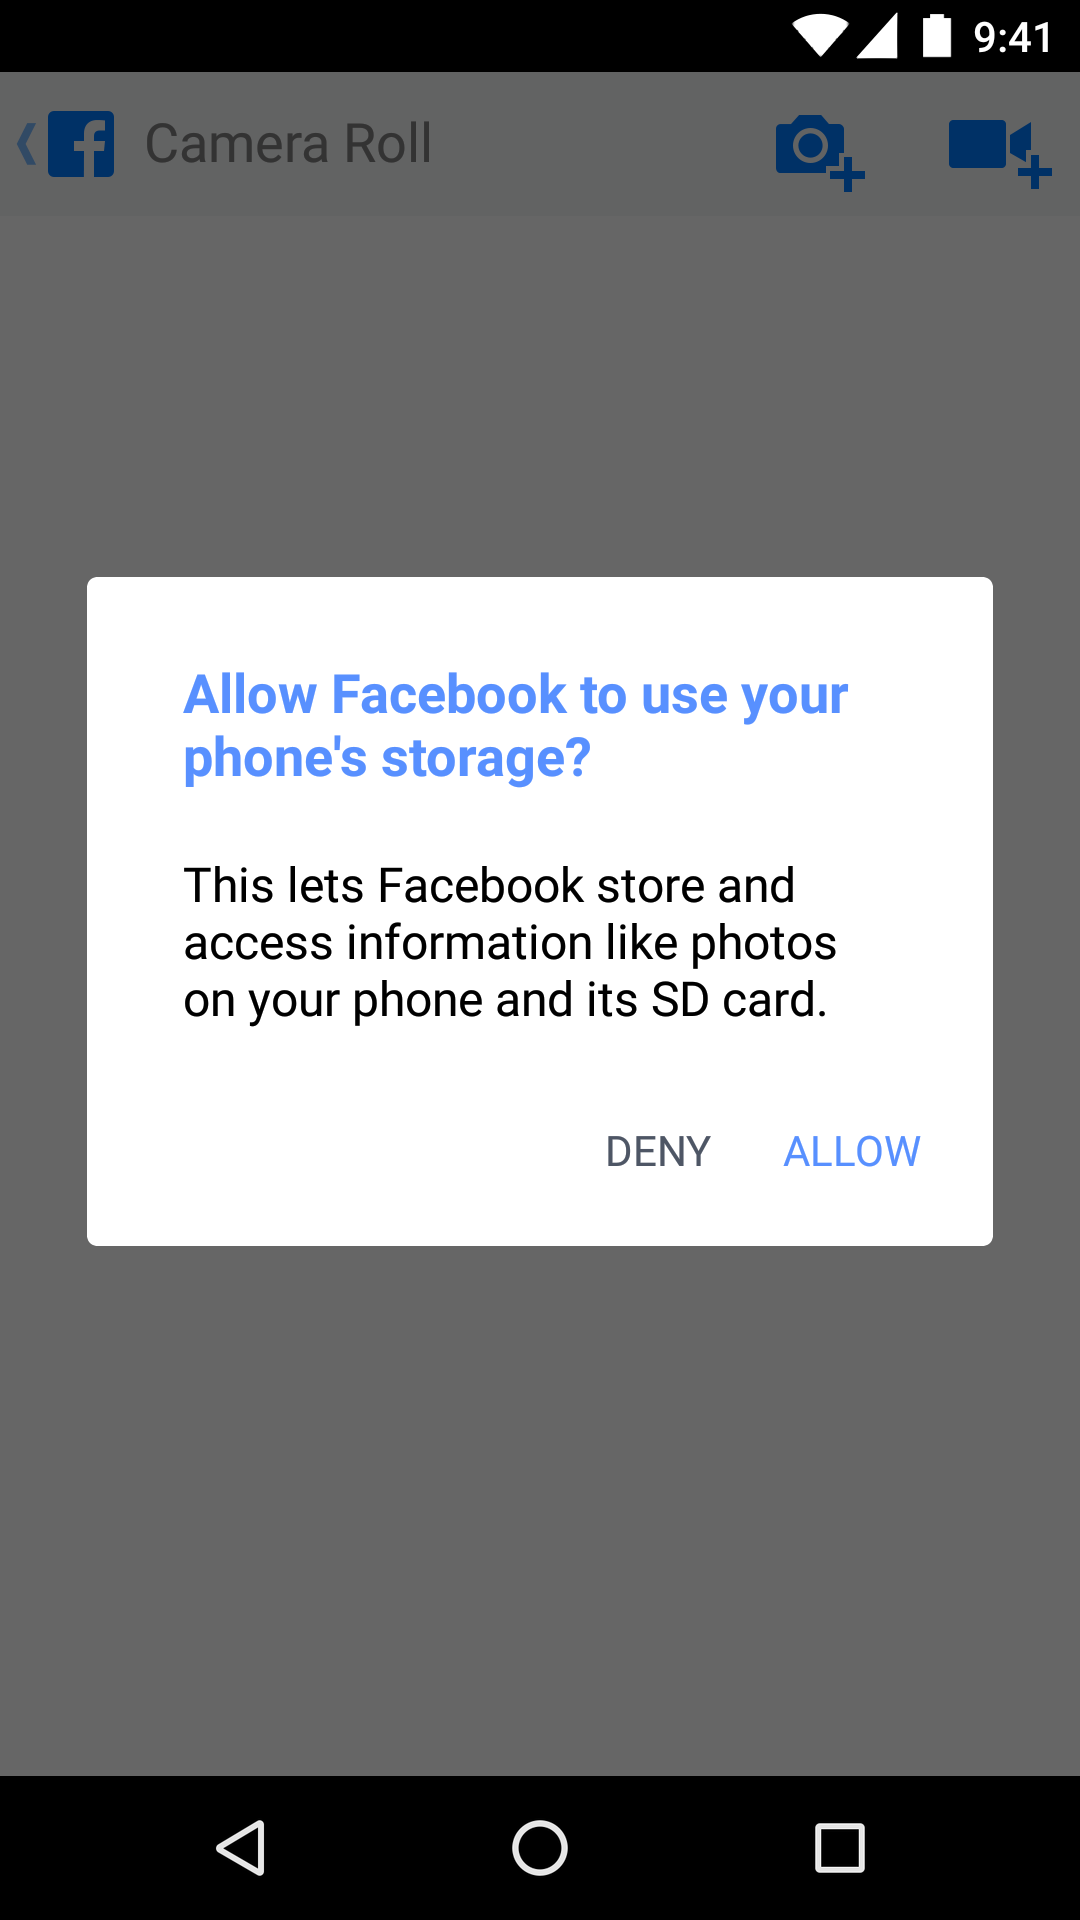
\includegraphics[width=\paperwidth]{../intro/facebook-perms-request}
        };
    \end{tikzpicture}
\end{frame}


\begin{frame}{malware defenses (3)}
    \begin{itemize}
        \item some email spam filters
        \item blacklists for web browsers
            \begin{itemize}
            \item Google Safe Browsing list (Chrome, Firefox)
            \item Microsoft SmartScreen (IE, Edge)
            \end{itemize}
    \end{itemize}
\end{frame}

\begin{frame}{malware counter-defenses}
    \begin{itemize}
    \item malware authors tries to make it hard-to-detect
    \item \myemph{obfuscation}:
        \begin{itemize}
        \item make code \myemph{harder to read}
        \item make code \myemph{different each time}
        \item \myemph{blend in} with normal files/applications/etc.
        \end{itemize}
    \end{itemize}
\end{frame}





